\documentclass[10pt,a4paper]{article}
\usepackage[utf8]{inputenc}
\usepackage[spanish]{babel}
\usepackage{amsmath}
\usepackage{amsfonts}
\usepackage{amssymb}
\usepackage{graphicx}
\usepackage{multicol}
\usepackage{titling}
\usepackage{titlesec}
\usepackage{array}
\usepackage{bm}
\usepackage{afterpage}
\usepackage{float}
\usepackage{graphicx}
\usepackage{epstopdf}
\usepackage{longtable}
\usepackage{xcolor}
\usepackage{epigraph} 
\setlength\epigraphwidth{1.5\textwidth}
\usepackage{subfigure}
\usepackage{anyfontsize}
\usepackage[left=2cm,right=2cm,top=2cm,bottom=2cm]{geometry}
\usepackage[colorlinks=true,
            linkcolor=blue,
            citecolor=blue,
            urlcolor=blue]{hyperref}

\begin{document}
\author{Benavides Wilmer, Farinango Luis,Velasco Angel}
\title{UNIVERSIDAD TÉCNICA DEL NORTE \\
FICA-CIERCOM\\
SISTEMAS EMBEBIDOS}
\maketitle
\begin{multicols}{2}
\section{Introducción}
Realizar una interfaz en el software de programación processing que permita presentar un juego de la anterior consola ATARI. Para ello, su palanca para dar movimiento al juego debe ser realizada por un arduino, botones y/o sensores.


\section{Objetivos} 
\subsection{Objetivo general}
Realizar la interfaz de juego 'Break Out' de la anterior consola ATARI programada en el software Processing.
\subsection{Objetivos específicos}
\begin{itemize}
\renewcommand{\labelitemi}{$-$}
\item Indagar sobre los diferentes juegos que tenía ATARI para así poder realizarlo en processing.
\item Analizar los diferentes métodos de programación en processing para el desarrollo de juegos.
\item Familiarizarce con la interacción entre processing y arduino.

\end{itemize}
\section{Marco Teórico}
\subsection{Processing}
Processing es un cuaderno de bocetos de software flexible y un lenguaje para aprender a codificar dentro del contexto de las artes visuales. Desde 2001, Processing ha promovido la alfabetización de software dentro de las artes visuales y la alfabetización visual dentro de la tecnología. Hay decenas de miles de estudiantes, artistas, diseñadores, investigadores y aficionados que usan Processing para aprender y crear prototipos.
\begin{figure}[H]
\centering

\includegraphics[scale=0.1]{proce.png}
\caption{Logotipo de processing}
\end{figure}




\subsection{Break Out}

En la parte inferior de la pantalla una rayita simulaba una raqueta de front-tenis que el jugador podía desplazar de izquierda a derecha. En la parte superior se situaba una banda conformada por rectángulos que simulaban ser ladrillos. Una pelota descendía de la nada y el jugador debía golpearla con la raqueta, entonces la pelota ascendía hasta pegar en el muro, los ladrillos tocados por la pelota desaparecían. La pelota volvía a descender y así sucesivamente. El objetivo del juego era terminar con la pared de ladrillos. 

\begin{figure}[H]
\centering
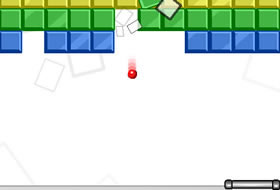
\includegraphics[scale=0.8]{brakout.jpg}
\caption{Break out }
\end{figure}
\end{multicols}


\section{Desarrollo}
\subsection{Diagrama de bloques}
Se muestra el proceso a seguir por medio de un diagrama de bloques.
\begin{figure}[H]
\centering
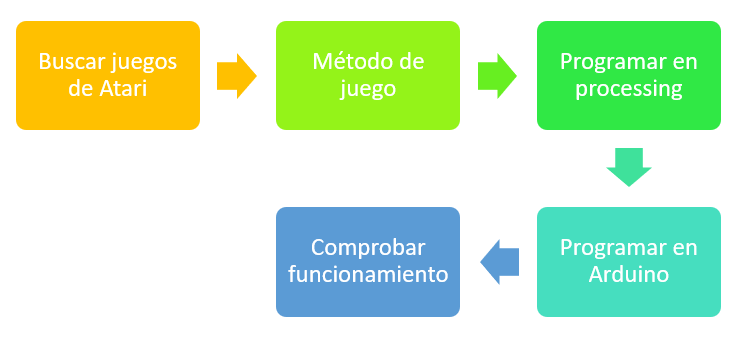
\includegraphics[scale=0.5]{proceso.PNG}
\caption{Diagrama de bloques}
\end{figure}




\subsection{Diseño arreglo de bloques}
Se genera un array donde se establece las dimensiones tanto de filas como columnas de los bloques a destruir. 

\begin{figure}[H]
\centering
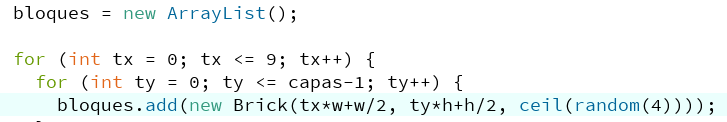
\includegraphics[scale=0.5]{arreglo de bloques.PNG}
\caption{array de bloques}
\end{figure}

\subsection{Diseño de la raqueta}
Mediante el uso de Arduino, se estable que el puerto COM 4 por donde se va a comunicar Arduino-Processing, se lee el valor y este mueve la raqueta en toda la dirección x.
\begin{figure}[H]
\centering
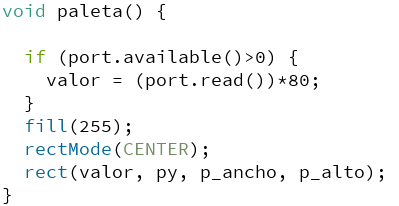
\includegraphics[scale=0.5]{raqueta.PNG}
\caption{Raqueta}
\end{figure}





\subsection{Diseño de pelota}
la pelota inicia en el centro y se incrementa su posición.
\begin{figure}[H]
\centering
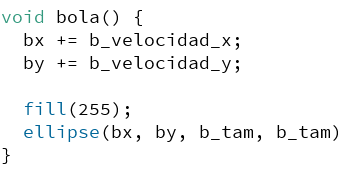
\includegraphics[scale=0.5]{bola.PNG}
\caption{Pelota}
\end{figure}




\subsection{Parámetros de control}
Para el control de la bola y la raqueta se compara el que si la bola llega a las dimensiones de la raqueta la bola rebota y sigue una trayectoria aleatoria.
Para los filos se limita tomando en cuenta las dimensiones de la ventana en ancho como largo con la ubicación de la bola.
\begin{figure}[H]
\centering
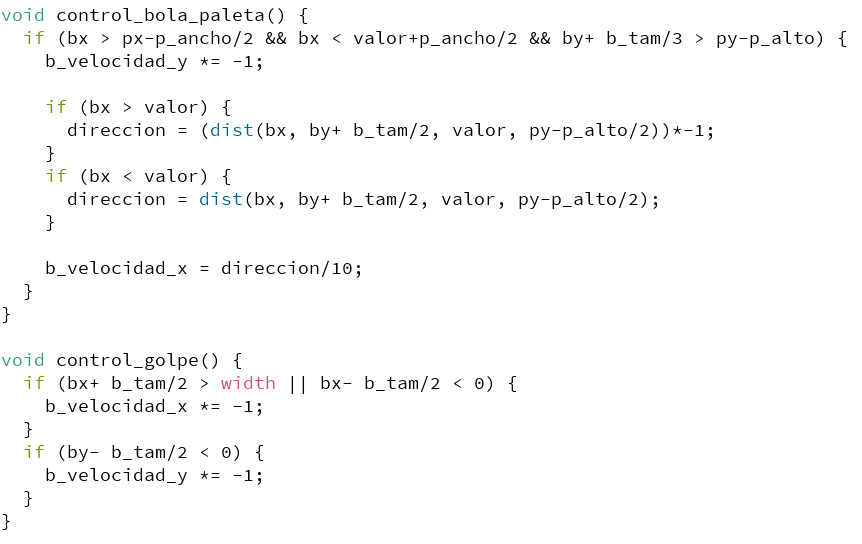
\includegraphics[scale=0.6]{control.PNG}
\caption{Control}
\end{figure}


\subsection{Parámetros para el ganador y perdedor}

Se compara si número de bloques existentes es igual a cero, si es así a ganado el juego.
\begin{figure}[H]
\centering
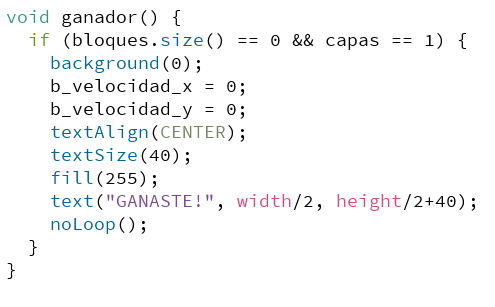
\includegraphics[scale=0.6]{ganador.PNG}
\caption{Ganador}
\end{figure}
Para perder se compara si la bola coincide con la ubicación de la raqueta, si no coincide pierde y vuelve a cero la ubicación de la bola.
\begin{figure}[H]
\centering
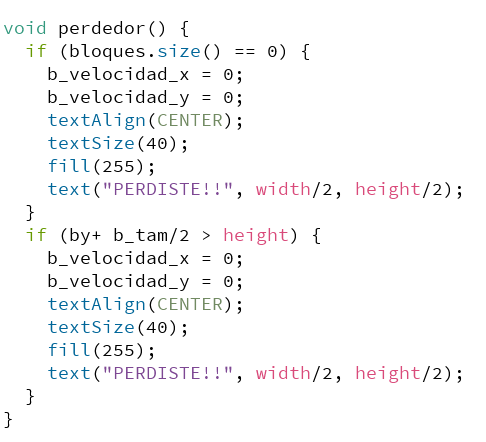
\includegraphics[scale=0.6]{perder.PNG}
\caption{código para el perdedor}
\end{figure}

\section{Resultados}
El circuito armado consta solamente de un potenciómetro que estará conectado al pin A1 del Arduino, este pin enviara datos analógicos que controlaran el movimiento del bloque del juego en cuestión.
\begin{figure}[H]
\centering
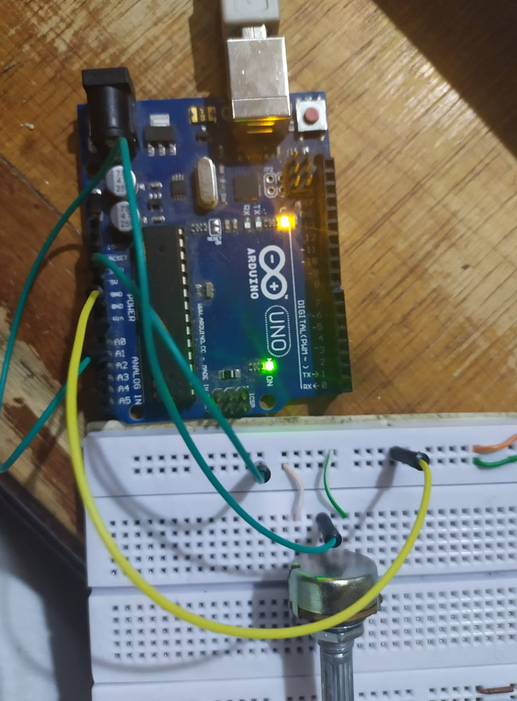
\includegraphics[scale=0.3]{circuito.PNG}
\caption{código para el perdedor}
\end{figure}
\begin{figure}[H]
\centering
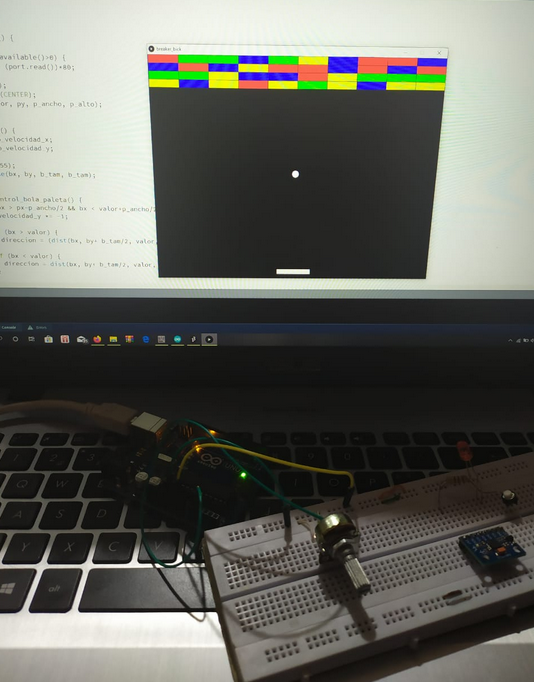
\includegraphics[scale=0.3]{funcio.PNG}
\caption{código para el perdedor}
\end{figure}

\section{Conclusiones y Recomendaciones}

\textbf{Conclusiones:}
\begin{itemize}
\renewcommand{\labelitemi}{$*$}
\item Una interfaz para un proyecto de un sistema embebido puede llegar a tener mucha importancia o protagonismo al momento de vender un producto o hacerlos más llamativo para el público o cliente.
\item Arduino tiene excelente compatibilidad con processing al manejar el mismo lenguaje de programación base, en este caso C++, aunque processing también es compatible con java.
\item La jerarqía entre los eventos de processing será la pieza clave para estructurar la programacion en este plataforma.
\end{itemize}

 
\textbf{Recomendaciones:}
\begin{itemize}
\item En la medida de lo posible tratar de tener el mínimo de interacciones entre processing y arduino, por el hecho de que suele haber interferencia en la transmisión de datos entre estas dos plataformas.
\item Se recomienda tener por lo menos conocimientos sobre fundamentos de programación en C++ y Java y una idea sobre programación orientada a objetos.
\item Identificar el puerto COM al que se conecta arduino en la PC es clave asignar los parámetros para la comunicación entre processing y arduino.
 
\end{itemize}
\section{Referencias Bibliográficas}

\begin{itemize}
\item Texas Intruments,(2019).CD74HCT4051 High-Speed CMOS Logic Analog Multiplexers and Demultiplexers.


\end{itemize}

\end{document}